\documentclass[aspectratio=169]{beamer}
\usepackage{lmodern}
%\usetheme{Madrid}
%\usecolortheme{giantoak}
\newcommand*\oldmacro{}
\let\oldmacro\insertshorttitle
\renewcommand*\insertshorttitle{\oldmacro\hfill\insertframenumber\,/\,\inserttotalframenumber}
\usepackage[framemethod=tikz]{mdframed}

%\usepackage{beamerthemesplit}
\usepackage{textpos}
\usepackage{pgf}
\usepackage{ulem}
%\logo{\pgfputat{\pgfxy(0,-.4)}{\pgfbox[right,base]{\includegraphics[height=1.0cm]{logo.jpg}}}}
%\newcommand{\nologo}{\setbeamertemplate{logo}{}}
\usepackage{booktabs}
\usepackage{graphicx}
\theoremstyle{principle}
\newtheorem*{principle}{Design Principle}


\titlegraphic{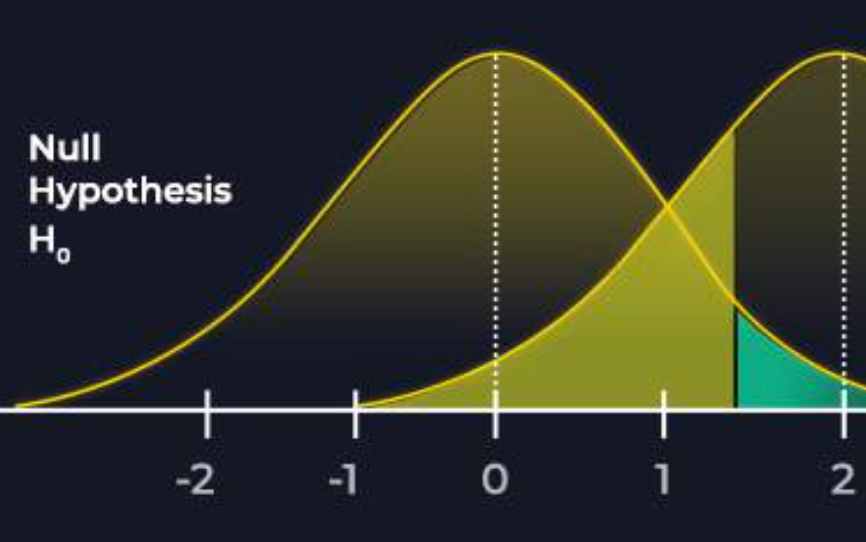
\includegraphics[width=1.0\paperwidth]{distros.png}}

\title{Amendments}
%\author[Jeremy Kedziora]{Wind Data Science Team\\
%\small{Uptake}}
\date{}

\begin{document}

%{
%%\nologo
%\begin{frame}
%    \maketitle
%\end{frame}
%}
%pages 1-7, 8-9, 14-15.


{
%  \usebackgroundtemplate{
\includegraphics[width=1.0\paperwidth]{statistics-review.jpg}}
  \usebackgroundtemplate{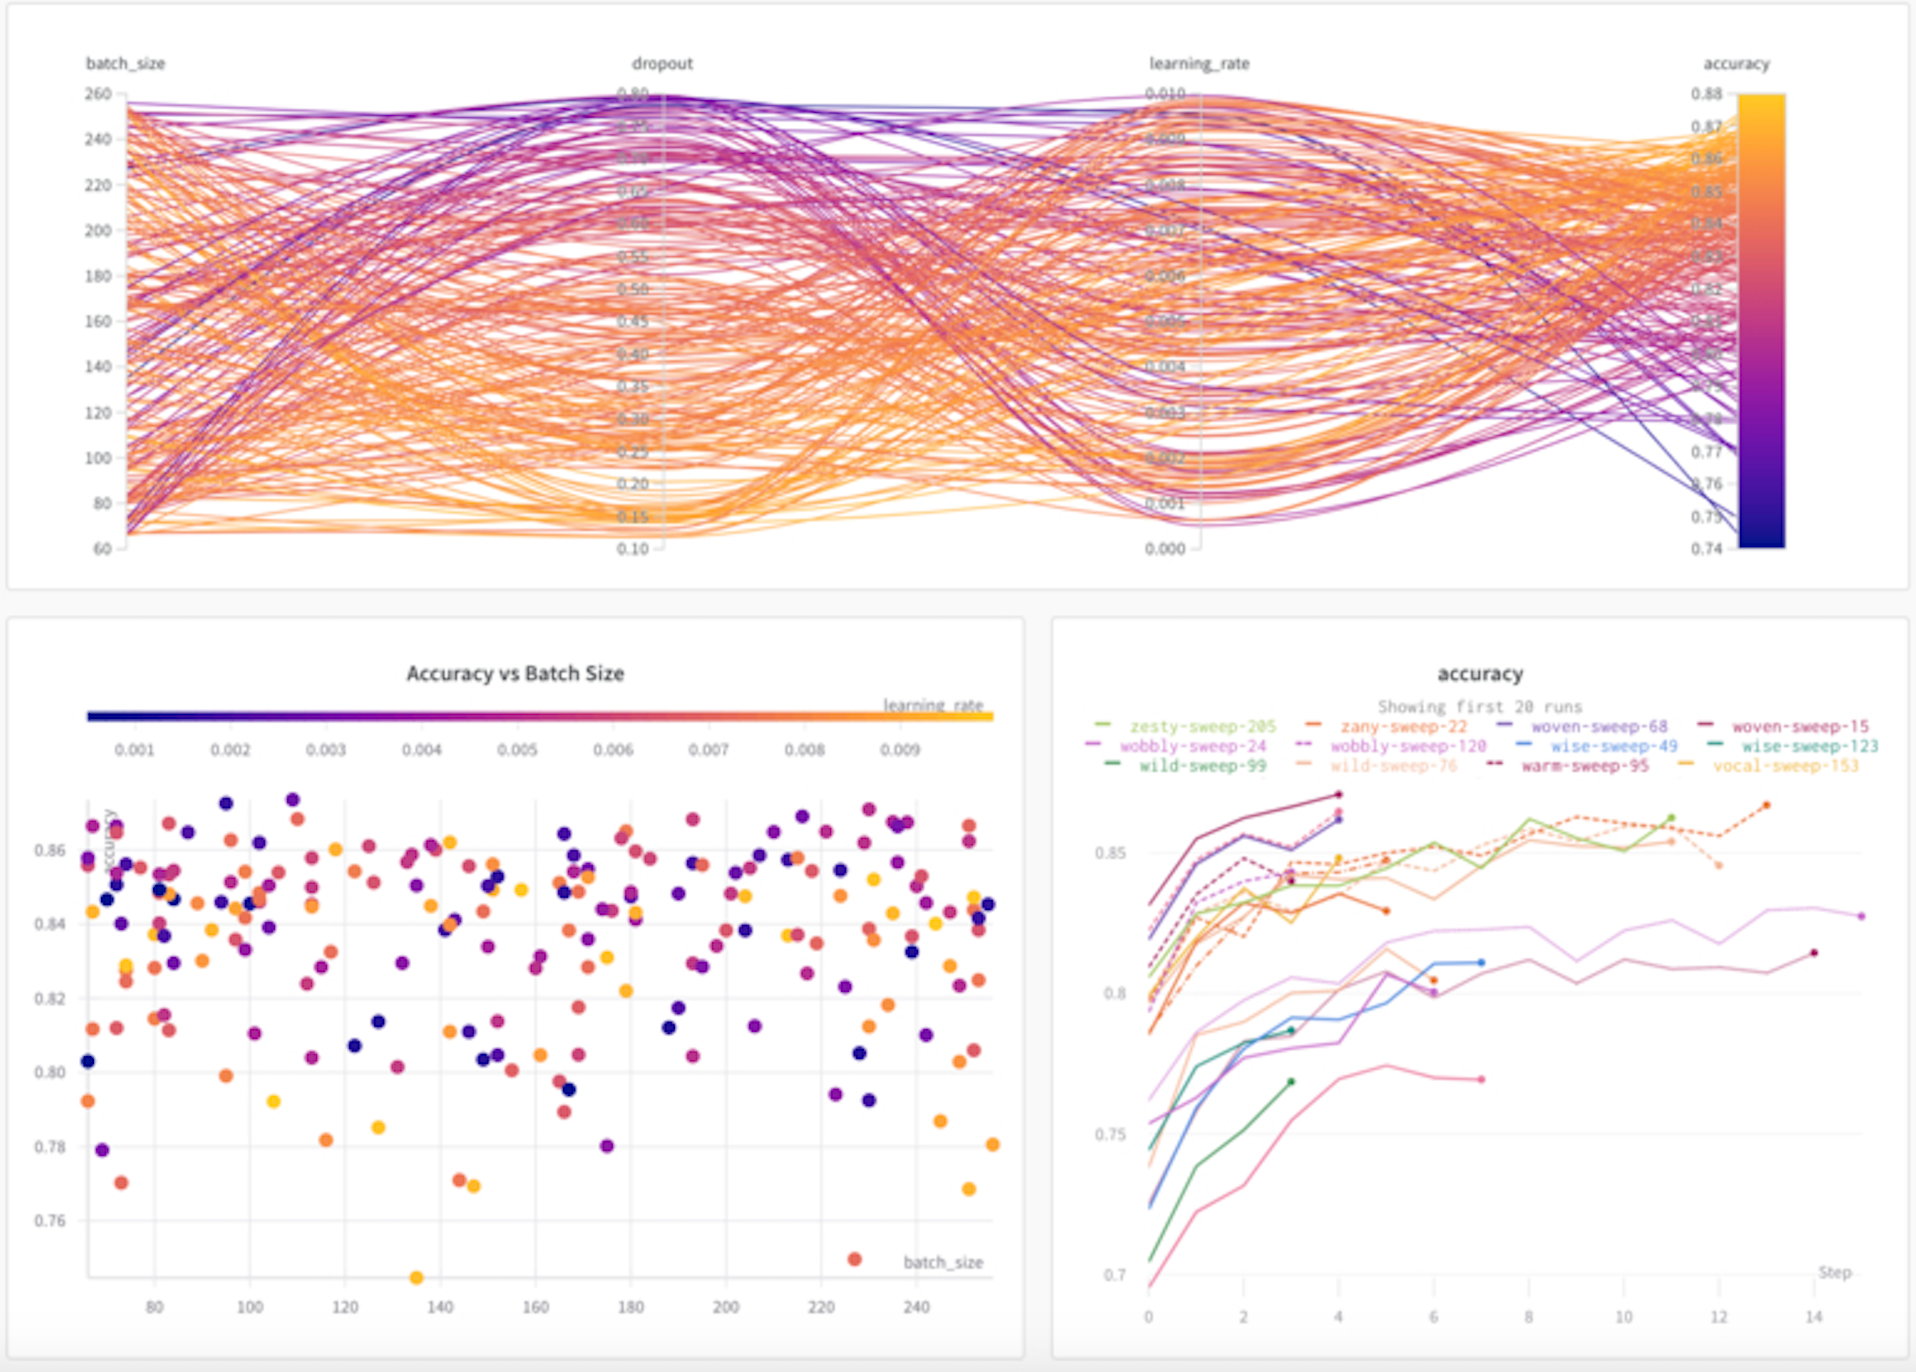
\includegraphics[scale=0.5]{ml_db.png}}
  \begin{frame}[plain]
  
\begin{mdframed}[tikzsetting={draw=white,fill=white,fill opacity=0.6,draw opacity=0.4,
               line width=0pt},backgroundcolor=none,leftmargin=20,
               rightmargin=20,innertopmargin=4pt]
\begin{center}
\Huge \textbf{Model Metrics}
\end{center}
\end{mdframed}

  \end{frame}
}

%most reliant on human cognition
%limited only by cognition
%hypothesis generating scheme often functioning as a gateway into more statistical analysis

%%@@@@@@@@@@@@@@@@@@@@@@@@@@@@@@@@@@@@@@@@@@@@@@@@@
%\begin{frame}
%\frametitle{Napoleon's Progress}
%\begin{center}
%
\includegraphics[scale=0.4]{experiment.png}
%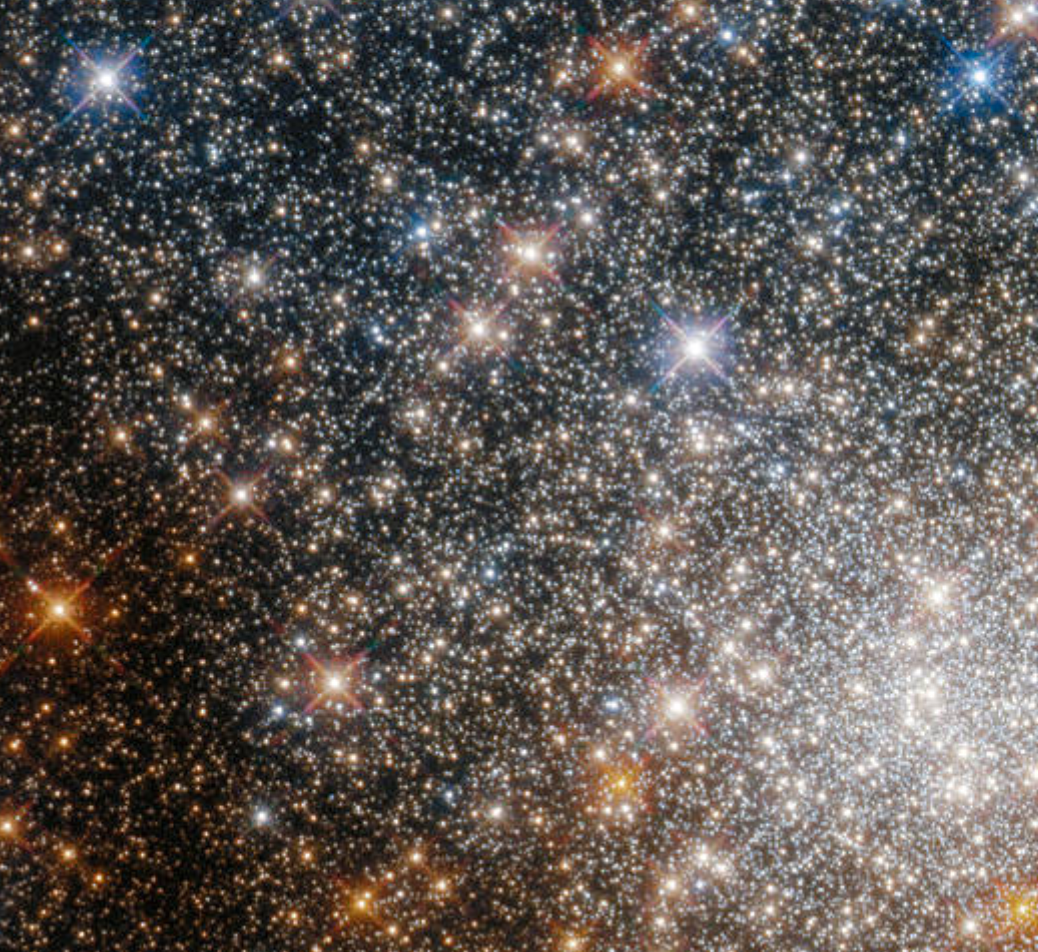
\includegraphics[scale=0.35]{stars.png}
%\end{center}
%
%\end{frame}

%@@@@@@@@@@@@@@@@@@@@@@@@@@@@@@@@@@@@@@@@@@@@@@@@@
\begin{frame}
\frametitle{Today:}

\begin{itemize}
\item Introduce metrics for linear regression;
\bigskip
\bigskip
\bigskip

\item Introduce metrics for binary dependent variables.

\end{itemize}

\end{frame}

%@@@@@@@@@@@@@@@@@@@@@@@@@@@@@@@@@@@@@@@@@@@@@@@@@
\begin{frame}

\begin{center}
\Huge\textbf{How good is the model?}\\
\end{center}

\end{frame}

%@@@@@@@@@@@@@@@@@@@@@@@@@@@@@@@@@@@@@@@@@@@@@@@@@
\begin{frame}

\begin{center}
\Huge\textbf{How well does the model predict?}\\
\end{center}

\end{frame}

%@@@@@@@@@@@@@@@@@@@@@@@@@@@@@@@@@@@@@@@@@@@@@@@@@
\begin{frame}
\frametitle{Linear Regresssion: Root Mean Squared Error}

\begin{columns}
\begin{column}{0.5\textwidth}

\begin{itemize}
\item We could measure model fit by looking at the `typical' error of the model when it makes predictions;
\bigskip

\item Remember how regression works?  It finds the $\beta$s by minimizing this:
\begin{align*}
\underbrace{\sum_i(\overbrace{y_i}^{\mbox{obs}} - \overbrace{(\beta_0 + \beta_1 x_i)}^{\mbox{prediction}})^2}_{\mbox{sum of squared residuals}}
\end{align*}

\item[] \color{white}\textbf{For HW7 root mean squared error: 3.390743.}
\end{itemize}

\end{column}
\begin{column}{0.5\textwidth}
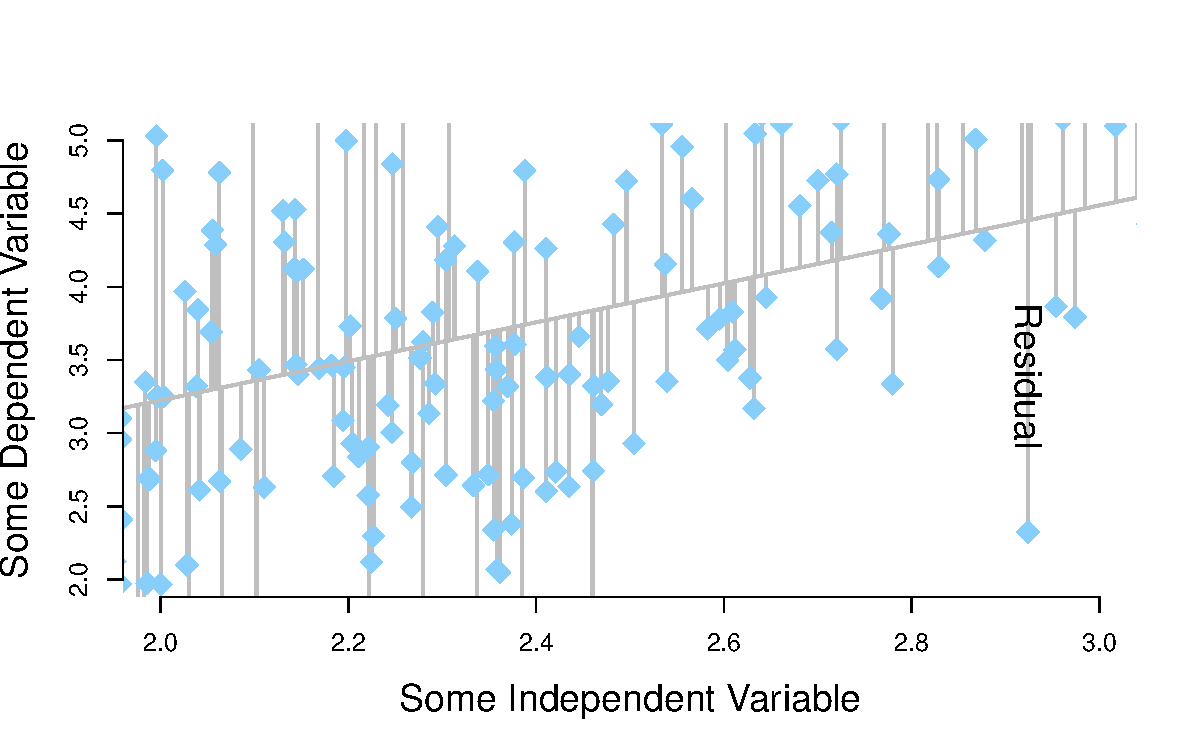
\includegraphics[scale=0.35]{point_cloud_line_zoomed_residuals.pdf}
\end{column}
\end{columns}

\end{frame}

%@@@@@@@@@@@@@@@@@@@@@@@@@@@@@@@@@@@@@@@@@@@@@@@@@
\begin{frame}
\frametitle{Linear Regresssion: Root Mean Squared Error}

\begin{columns}
\begin{column}{0.5\textwidth}

\begin{itemize}
\item We could measure model fit by looking at the `typical' error of the model when it makes predictions;
\bigskip

\item Remember how regression works?  It finds the $\beta$s by minimizing this:
\begin{align*}
\underbrace{\sum_i(\overbrace{y_i}^{\mbox{obs}} - \overbrace{(\beta_0 + \beta_1 x_i)}^{\mbox{prediction}})^2}_{\mbox{total squared error}}
\end{align*}

\item[] \color{white} \textbf{For HW7 root mean squared error: 3.390743.}
\end{itemize}

\end{column}
\begin{column}{0.5\textwidth}
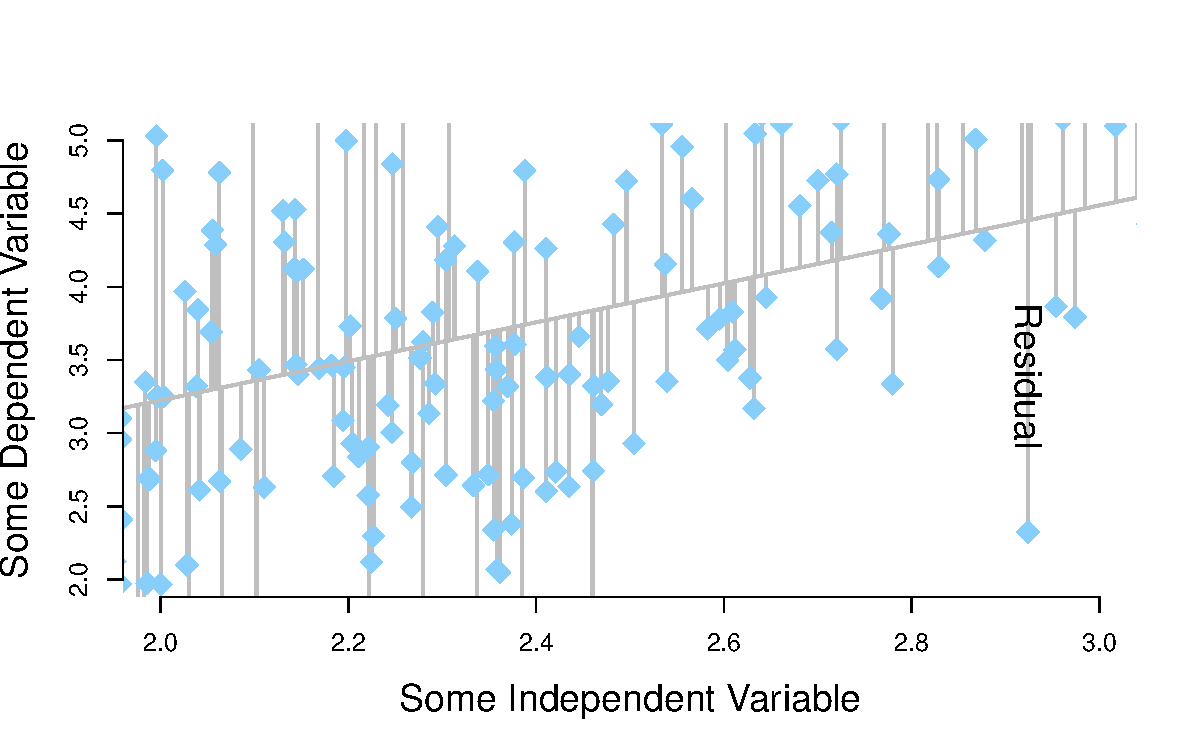
\includegraphics[scale=0.35]{point_cloud_line_zoomed_residuals.pdf}
\end{column}
\end{columns}

\end{frame}

%@@@@@@@@@@@@@@@@@@@@@@@@@@@@@@@@@@@@@@@@@@@@@@@@@
\begin{frame}
\frametitle{Linear Regresssion: Root Mean Squared Error}

\begin{columns}
\begin{column}{0.5\textwidth}

\begin{itemize}
\item We could measure model fit by looking at the `typical' error of the model when it makes predictions;
\bigskip

\item Remember how regression works?  It finds the $\beta$s by minimizing this:
\begin{align*}
\underbrace{\frac{1}{n}\sum_i(\overbrace{y_i}^{\mbox{obs}} - \overbrace{(\beta_0 + \beta_1 x_i)}^{\mbox{prediction}})^2}_{\mbox{mean squared error}}
\end{align*}

\item[] \color{white} \textbf{For HW7 root mean squared error: 3.390743.}
\end{itemize}

\end{column}
\begin{column}{0.5\textwidth}
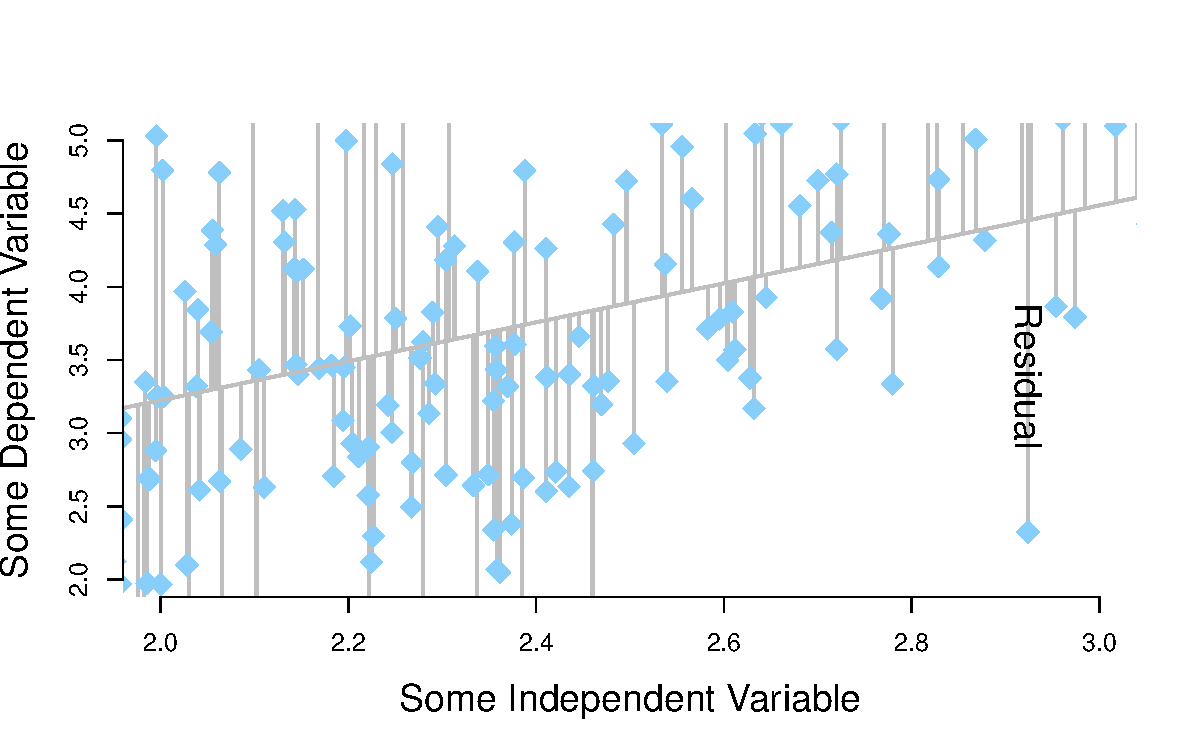
\includegraphics[scale=0.35]{point_cloud_line_zoomed_residuals.pdf}
\end{column}
\end{columns}

\end{frame}

%@@@@@@@@@@@@@@@@@@@@@@@@@@@@@@@@@@@@@@@@@@@@@@@@@
\begin{frame}
\frametitle{Linear Regresssion: Root Mean Squared Error}

\begin{columns}
\begin{column}{0.5\textwidth}

\begin{itemize}
\item We could measure model fit by looking at the `typical' error of the model when it makes predictions;
\bigskip

\item Remember how regression works?  It finds the $\beta$s by minimizing this:
\begin{align*}
\underbrace{\sqrt{\frac{1}{n}\sum_i(\overbrace{y_i}^{\mbox{obs}} - \overbrace{(\beta_0 + \beta_1 x_i)}^{\mbox{prediction}})^2}}_{\mbox{root mean squared error}}
\end{align*}

\item[] \color{white} \textbf{For HW7 root mean squared error: 3.390743.}
\end{itemize}

\end{column}
\begin{column}{0.5\textwidth}
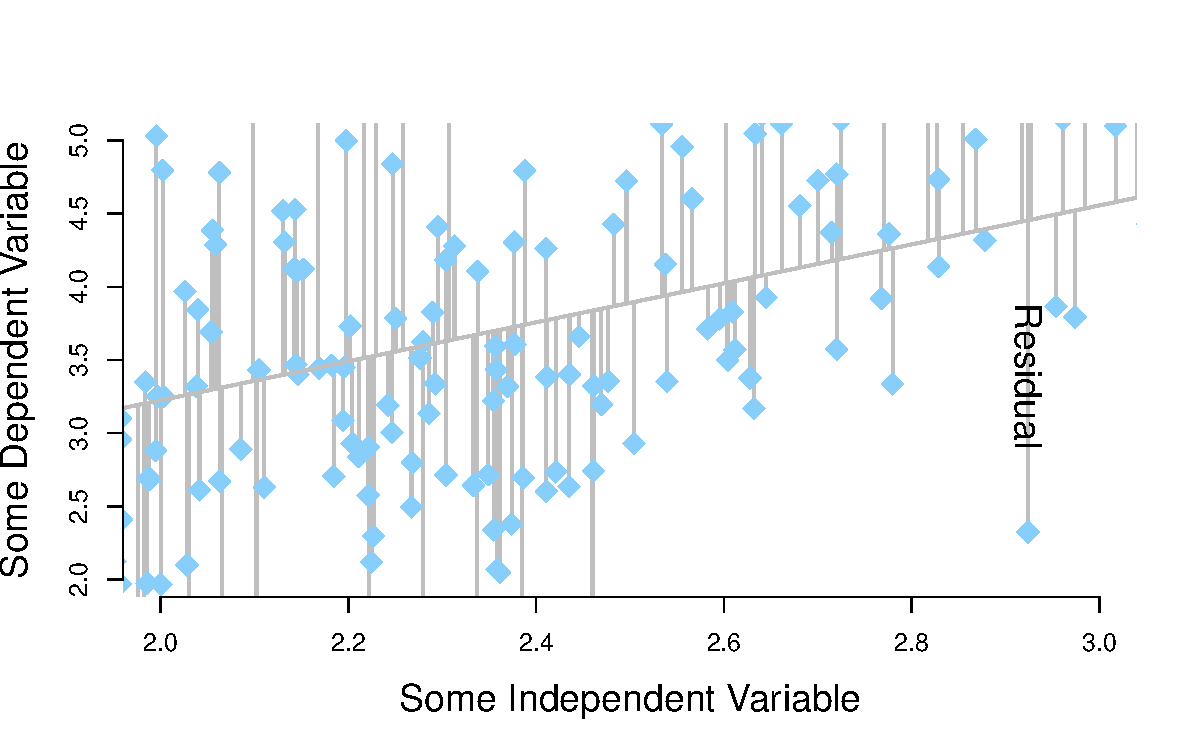
\includegraphics[scale=0.35]{point_cloud_line_zoomed_residuals.pdf}
\end{column}
\end{columns}

\end{frame}

%@@@@@@@@@@@@@@@@@@@@@@@@@@@@@@@@@@@@@@@@@@@@@@@@@
\begin{frame}
\frametitle{Linear Regresssion: Root Mean Squared Error}

\begin{columns}
\begin{column}{0.5\textwidth}

\begin{itemize}
\item We could measure model fit by looking at the `typical' error of the model when it makes predictions;
\bigskip

\item Remember how regression works?  It finds the $\beta$s by minimizing this:
\begin{align*}
\underbrace{\sqrt{\frac{1}{n}\sum_i(\overbrace{y_i}^{\mbox{obs}} - \overbrace{(\beta_0 + \beta_1 x_i)}^{\mbox{prediction}})^2}}_{\mbox{root mean squared error}}
\end{align*}

\item \textbf{For HW7 root mean squared error: 3.3907 years.}
\end{itemize}

\end{column}
\begin{column}{0.5\textwidth}

% latex table generated in R 4.1.1 by xtable 1.8-4 package
% Sun Nov 27 14:49:22 2022
\begin{table}[ht]
\centering
\begin{tabular}{rrr}
  \hline
   \hline
 & Estimate & Pr($>$$|$t$|$) \\ 
  \hline
   \hline
Intercept & 62.3701 & 0.0000 \\ 
  health exp \% GDP & 0.1993 & 0.0567 \\ 
  log(GNI PC) & 1.4278 & 0.0001 \\ 
  infant mortality & -0.2288 & 0.0000 \\ 
   \hline
   \hline
   &&\\
\end{tabular}\\
\color{white}Multiple R-squared:  0.8854\\ 
$F$-statistic: $p$-value: $<$ 2.2e-16
\end{table}

\end{column}
\end{columns}

\end{frame}

%@@@@@@@@@@@@@@@@@@@@@@@@@@@@@@@@@@@@@@@@@@@@@@@@@
\begin{frame}
\frametitle{Linear regression: $R^2$}

\begin{columns}
\begin{column}{0.5\textwidth}

\begin{itemize}
\item We could measure model fit by comparing:
\begin{itemize}
\item `Typical' model prediction error;
\item Error associated with just predicting the mean of the dependent variable;
 \end{itemize}
\bigskip

\item One way to do this would be:
\begin{align*}
R^2 = 1 - \frac{\mbox{sum of squared residuals}}{\mbox{error from predicting mean}}
\end{align*}

\item[] \color{white}Beware!  $R^2$ will always increase as you add more independent variables.
\end{itemize}

\end{column}
\begin{column}{0.5\textwidth}



\end{column}
\end{columns}

\end{frame}

%@@@@@@@@@@@@@@@@@@@@@@@@@@@@@@@@@@@@@@@@@@@@@@@@@
\begin{frame}
\frametitle{Linear regression: $R^2$}

\begin{columns}
\begin{column}{0.5\textwidth}

\begin{itemize}
\item We could measure model fit by comparing:
\begin{itemize}
\item `Typical' model prediction error;
\item Error associated with just predicting the mean of the dependent variable;
 \end{itemize}
\bigskip

\item One way to do this would be:
\begin{align*}
R^2 = 1 - \frac{\mbox{\textbf{sum of squared residuals}}}{\mbox{error from predicting mean}}
\end{align*}

\item[] \color{white}Beware!  $R^2$ will always increase as you add more independent variables.
\end{itemize}

\end{column}
\begin{column}{0.5\textwidth}

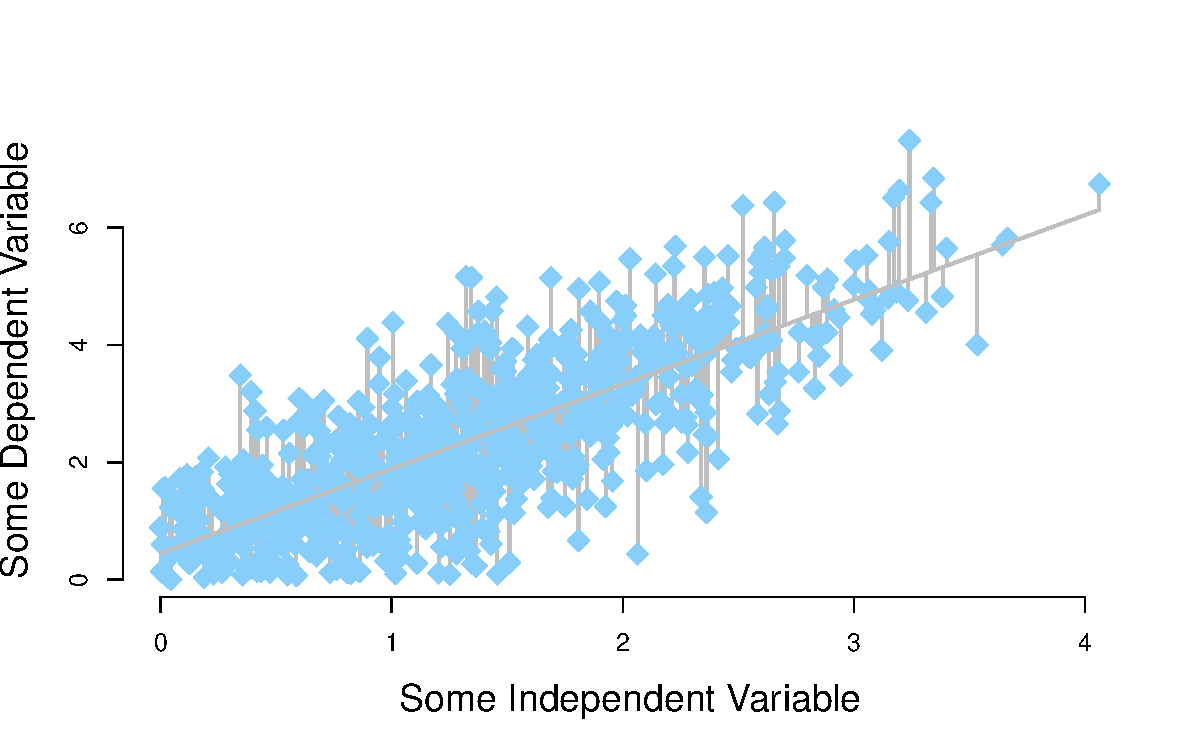
\includegraphics[scale=0.35]{point_cloud_line_residual.pdf}

\end{column}
\end{columns}

\end{frame}

%@@@@@@@@@@@@@@@@@@@@@@@@@@@@@@@@@@@@@@@@@@@@@@@@@
\begin{frame}
\frametitle{Linear regression: $R^2$}

\begin{columns}
\begin{column}{0.5\textwidth}

\begin{itemize}
\item We could measure model fit by comparing:
\begin{itemize}
\item `Typical' model prediction error;
\item Error associated with just predicting the mean of the dependent variable;
 \end{itemize}
\bigskip

\item One way to do this would be:
\begin{align*}
R^2 = 1 - \frac{\mbox{sum of squared residuals}}{\mbox{\textbf{error from predicting mean}}}
\end{align*}

\item[] \color{white}Beware!  $R^2$ will always increase as you add more independent variables.
\end{itemize}

\end{column}
\begin{column}{0.5\textwidth}

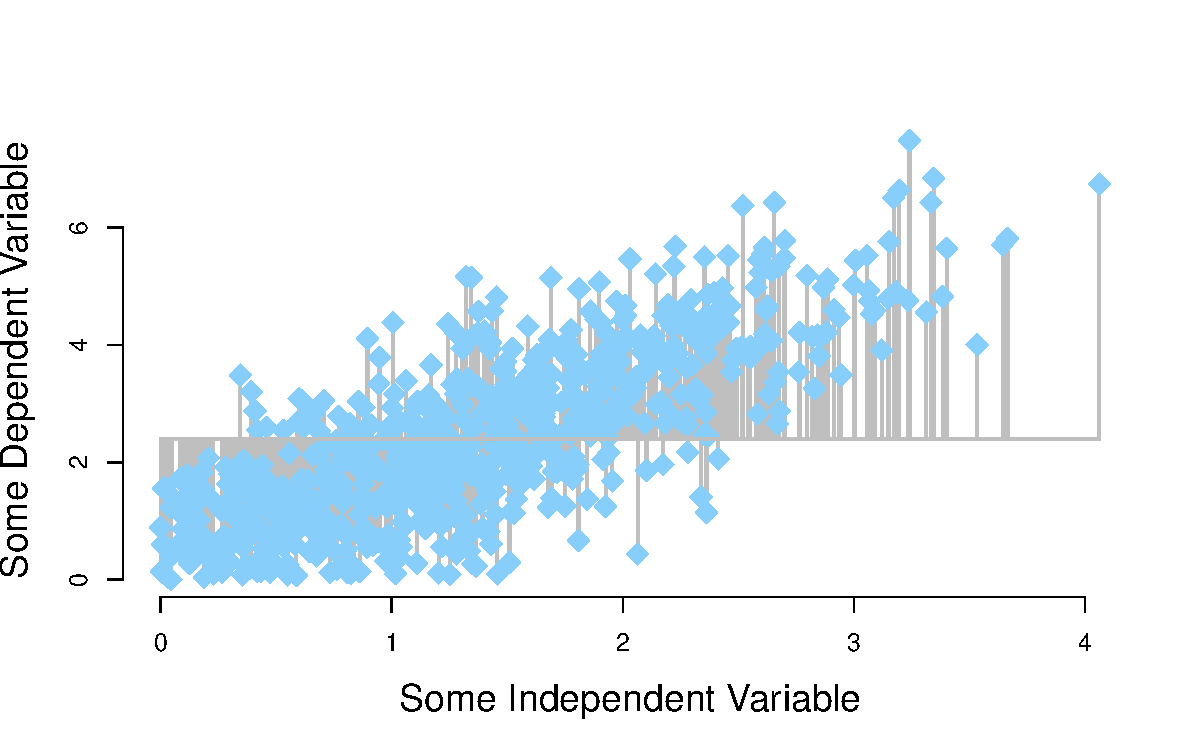
\includegraphics[scale=0.35]{point_cloud_mean_residual.pdf}

\end{column}
\end{columns}

\end{frame}

%@@@@@@@@@@@@@@@@@@@@@@@@@@@@@@@@@@@@@@@@@@@@@@@@@
\begin{frame}
\frametitle{Linear regression: $R^2$}

\begin{columns}
\begin{column}{0.5\textwidth}

\begin{itemize}
\item We could measure model fit by comparing:
\begin{itemize}
\item `Typical' model prediction error;
\item Error associated with just predicting the mean of the dependent variable;
 \end{itemize}
\bigskip

\item One way to do this would be:
\begin{align*}
R^2 = 1 - \frac{\mbox{sum of squared residuals}}{\mbox{error from predicting mean}}
\end{align*}

\item[] \color{white}Beware!  $R^2$ will always increase as you add more independent variables.

\end{itemize}

\end{column}
\begin{column}{0.5\textwidth}

% latex table generated in R 4.1.1 by xtable 1.8-4 package
% Sun Nov 27 14:49:22 2022
\begin{table}[ht]
\centering
\begin{tabular}{rrr}
  \hline
   \hline
 & Estimate & Pr($>$$|$t$|$) \\ 
  \hline
   \hline
Intercept & 62.3701 & 0.0000 \\ 
  health exp \% GDP & 0.1993 & 0.0567 \\ 
  log(GNI PC) & 1.4278 & 0.0001 \\ 
  infant mortality & -0.2288 & 0.0000 \\ 
   \hline
   \hline
   &&\\
\end{tabular}\\
Multiple R-squared:  0.8854\\ 
\color{white}$F$-statistic: $p$-value: $<$ 2.2e-16
\end{table}

\end{column}
\end{columns}

\end{frame}

%@@@@@@@@@@@@@@@@@@@@@@@@@@@@@@@@@@@@@@@@@@@@@@@@@
\begin{frame}
\frametitle{Linear regression: $R^2$}

\begin{columns}
\begin{column}{0.5\textwidth}

\begin{itemize}
\item We could measure model fit by comparing:
\begin{itemize}
\item `Typical' model prediction error;
\item Error associated with just predicting the mean of the dependent variable;
 \end{itemize}
\bigskip

\item One way to do this would be:
\begin{align*}
R^2 = 1 - \frac{\mbox{sum of squared residuals}}{\mbox{error from predicting mean}}
\end{align*}

\item Beware!  $R^2$ will always increase as you add more independent variables.

\end{itemize}

\end{column}
\begin{column}{0.5\textwidth}

% latex table generated in R 4.1.1 by xtable 1.8-4 package
% Sun Nov 27 14:49:22 2022
\begin{table}[ht]
\centering
\begin{tabular}{rrr}
  \hline
   \hline
 & Estimate & Pr($>$$|$t$|$) \\ 
  \hline
   \hline
Intercept & 62.3701 & 0.0000 \\ 
  health exp \% GDP & 0.1993 & 0.0567 \\ 
  log(GNI PC) & 1.4278 & 0.0001 \\ 
  infant mortality & -0.2288 & 0.0000 \\ 
   \hline
   \hline
   &&\\
\end{tabular}\\
Multiple R-squared:  0.8854\\ 
\color{white}$F$-statistic: $p$-value: $<$ 2.2e-16
\end{table}

\end{column}
\end{columns}

\end{frame}

%@@@@@@@@@@@@@@@@@@@@@@@@@@@@@@@@@@@@@@@@@@@@@@@@@
\begin{frame}
\frametitle{Linear Regression: $F$-test}

\begin{columns}
\begin{column}{0.5\textwidth}

\begin{itemize}
\item We could measure model fit by doing hypothesis testing;
\bigskip
\bigskip

\item Given a model with some independent variables ask does the model fit the data well?
\begin{itemize}
\item $\mathbf{H_0}$: \color{white}The fit of the `intercept-only' model is no different than the fit of the `intercept-plus-variables' model;\color{black}
\item $\mathbf{H_A}$: \color{white}The fit of the `intercept-only' model is significantly worse;\color{black}
\item \textbf{Test stat}: \color{white}$F$-statistic -- measures the variation in the dependent variable explained by the model;\color{black}
\item \textbf{Rejection criterion}: \color{white}$p$-value < 0.05.
\end{itemize}


\end{itemize}

\end{column}
\begin{column}{0.5\textwidth}

% latex table generated in R 4.1.1 by xtable 1.8-4 package
% Sun Nov 27 14:49:22 2022
\begin{table}[ht]
\centering
\begin{tabular}{rrr}
  \hline
   \hline
 & Estimate & Pr($>$$|$t$|$) \\ 
  \hline
   \hline
Intercept & 62.3701 & 0.0000 \\ 
  health exp \% GDP & 0.1993 & 0.0567 \\ 
  log(GNI PC) & 1.4278 & 0.0001 \\ 
  infant mortality & -0.2288 & 0.0000 \\ 
   \hline
   \hline
   &&\\
\end{tabular}\\
Multiple R-squared:  0.8854\\ 
\color{white}$F$-statistic: $p$-value: $<$ 2.2e-16
\end{table}

\end{column}
\end{columns}

\end{frame}

%@@@@@@@@@@@@@@@@@@@@@@@@@@@@@@@@@@@@@@@@@@@@@@@@@
\begin{frame}
\frametitle{Linear Regression: $F$-test}

\begin{columns}
\begin{column}{0.5\textwidth}

\begin{itemize}
\item We could measure model fit by doing hypothesis testing;
\bigskip
\bigskip

\item Given a model with some independent variables ask does the model fit the data well?
\begin{itemize}
\item $\mathbf{H_0}$: The fit of the `intercept-only' model is no different than the fit of the `intercept-plus-variables' model;
\item $\mathbf{H_A}$: The fit of the `intercept-only' model is significantly worse;
\item \textbf{Test stat}: \color{white}$F$-statistic -- measures the variation in the dependent variable explained by the model;\color{black}
\item \textbf{Rejection criterion}: \color{white}$p$-value < 0.05.
\end{itemize}


\end{itemize}

\end{column}
\begin{column}{0.5\textwidth}

% latex table generated in R 4.1.1 by xtable 1.8-4 package
% Sun Nov 27 14:49:22 2022
\begin{table}[ht]
\centering
\begin{tabular}{rrr}
  \hline
   \hline
 & Estimate & Pr($>$$|$t$|$) \\ 
  \hline
   \hline
Intercept & 62.3701 & 0.0000 \\ 
  health exp \% GDP & 0.1993 & 0.0567 \\ 
  log(GNI PC) & 1.4278 & 0.0001 \\ 
  infant mortality & -0.2288 & 0.0000 \\ 
   \hline
   \hline
   &&\\
\end{tabular}\\
Multiple R-squared:  0.8854\\ 
\color{white}$F$-statistic: $p$-value: $<$ 2.2e-16
\end{table}

\end{column}
\end{columns}

\end{frame}

%@@@@@@@@@@@@@@@@@@@@@@@@@@@@@@@@@@@@@@@@@@@@@@@@@
\begin{frame}
\frametitle{Linear Regression: $F$-test}

\begin{columns}
\begin{column}{0.5\textwidth}

\begin{itemize}
\item We could measure model fit by doing hypothesis testing;
\bigskip
\bigskip

\item Given a model with some independent variables ask does the model fit the data well?
\begin{itemize}
\item $\mathbf{H_0}$: The fit of the `intercept-only' model is no different than the fit of the `intercept-plus-variables' model;
\item $\mathbf{H_A}$: The fit of the `intercept-only' model is significantly worse;
\item \textbf{Test stat}: $F$-statistic -- measures the variation in the dependent variable explained by the model;
\item \textbf{Rejection criterion}: $p$-value $< 0.05$.
\end{itemize}


\end{itemize}

\end{column}
\begin{column}{0.5\textwidth}

% latex table generated in R 4.1.1 by xtable 1.8-4 package
% Sun Nov 27 14:49:22 2022
\begin{table}[ht]
\centering
\begin{tabular}{rrr}
  \hline
   \hline
 & Estimate & Pr($>$$|$t$|$) \\ 
  \hline
   \hline
Intercept & 62.3701 & 0.0000 \\ 
  health exp \% GDP & 0.1993 & 0.0567 \\ 
  log(GNI PC) & 1.4278 & 0.0001 \\ 
  infant mortality & -0.2288 & 0.0000 \\ 
   \hline
   \hline
   &&\\
\end{tabular}\\
Multiple R-squared:  0.8854\\ 
\color{white}$F$-statistic: $p$-value: $<$ 2.2e-16
\end{table}

\end{column}
\end{columns}

\end{frame}

%@@@@@@@@@@@@@@@@@@@@@@@@@@@@@@@@@@@@@@@@@@@@@@@@@
\begin{frame}
\frametitle{Linear Regression: $F$-test}

\begin{columns}
\begin{column}{0.5\textwidth}

\begin{itemize}
\item We could measure model fit by doing hypothesis testing;
\bigskip
\bigskip

\item Given a model with some independent variables ask does the model fit the data well?
\begin{itemize}
\item $\mathbf{H_0}$: The fit of the `intercept-only' model is no different than the fit of the `intercept-plus-variables' model;
\item $\mathbf{H_A}$: The fit of the `intercept-only' model is significantly worse;
\item \textbf{Test stat}: $F$-statistic -- measures the variation in the dependent variable explained by the model;
\item \textbf{Rejection criterion}: $p$-value $< 0.05$.
\end{itemize}


\end{itemize}

\end{column}
\begin{column}{0.5\textwidth}

% latex table generated in R 4.1.1 by xtable 1.8-4 package
% Sun Nov 27 14:49:22 2022
\begin{table}[ht]
\centering
\begin{tabular}{rrr}
  \hline
   \hline
 & Estimate & Pr($>$$|$t$|$) \\ 
  \hline
   \hline
Intercept & 62.3701 & 0.0000 \\ 
  health exp \% GDP & 0.1993 & 0.0567 \\ 
  log(GNI PC) & 1.4278 & 0.0001 \\ 
  infant mortality & -0.2288 & 0.0000 \\ 
   \hline
   \hline
   &&\\
\end{tabular}\\
Multiple R-squared:  0.8854\\ 
$F$-statistic: $p$-value: $<$ 2.2e-16
\end{table}

\end{column}
\end{columns}

\end{frame}

%@@@@@@@@@@@@@@@@@@@@@@@@@@@@@@@@@@@@@@@@@@@@@@@@@
\begin{frame}
\frametitle{Logistic Regression: predictions?}

\begin{itemize}
\item A logit actually outputs a \textbf{predicted probability} when it makes a prediction;
\bigskip
\bigskip

\item To turn a predicted probability into a \textbf{predicted value}:
\begin{itemize}
\item Choose a threshold $t$;
\item If predicted probability $> t$ then predict a 1;
\item If predicted probability $< t$ then predict a 0;
\end{itemize}
\bigskip
\bigskip

\item Once we have predicted values we can start to assess model fit:
\begin{itemize}
\item \textbf{True Positive}: model predicts 1, actual observation is 1;
\item \textbf{True Negative}: model predicts 0, actual observation is 0;
\item \textbf{False Positive}: model predicts 1, actual observation is 0;
\item \textbf{False Negative}: model predicts 0, actual observation is 1.
\end{itemize}

\end{itemize}

\end{frame}

%@@@@@@@@@@@@@@@@@@@@@@@@@@@@@@@@@@@@@@@@@@@@@@@@@
\begin{frame}
\frametitle{Logistic Regression: predictions?}

Note: everything to follow will reference the Titanic example from the logistic regression lecture.
\bigskip
% latex table generated in R 3.5.1 by xtable 1.8-3 package
% Sun Mar 10 22:01:57 2019
\begin{table}[ht]
\centering
\begin{tabular}{rrrrr}
  \hline
    \hline
 & Estimate & Std. Error & z value & Pr($>$$|$z$|$) \\ 
  \hline
    \hline
(Intercept) & 5.2973 & 0.5574 & 9.50 & 0.0000 \\ 
  Pclass & -1.1777 & 0.1461 & -8.06 & 0.0000 \\ 
  Age & -0.0435 & 0.0077 & -5.63 & 0.0000 \\ 
  Male & -2.7573 & 0.2004 & -13.76 & 0.0000 \\ 
  Siblings/Spouses & -0.4018 & 0.1107 & -3.63 & 0.0003 \\ 
  Parents/Children & -0.1065 & 0.1186 & -0.90 & 0.3691 \\ 
  Fare & 0.0028 & 0.0024 & 1.17 & 0.2437 \\ 
   \hline
     \hline
\end{tabular}
\end{table}

\end{frame}

%@@@@@@@@@@@@@@@@@@@@@@@@@@@@@@@@@@@@@@@@@@@@@@@@@
\begin{frame}
\frametitle{Logistic Regression: predictions?  Choose a threshold $t$}

% latex table generated in R 4.1.1 by xtable 1.8-4 package
% Tue Nov 29 16:11:16 2022
\begin{table}[ht]
\centering
\begin{tabular}{l | r | c | c | c}

 Name & Survived & Predicted & Predicted &Type\\ 
&&Probability&Value\\
  \hline
  \hline
 Mr. Owen Harris Braund &   0 & 0.09 &&\\ 
 Mrs. John Bradley Cumings &   1 & 0.91 &&\\ 
 Miss. Laina Heikkinen &   1 & 0.66 &&\\ 
 Mrs. Jacques Heath Futrelle &   1 & 0.91 &&\\ 
 Mr. William Henry Allen &   0 & 0.08 &&\\ 
 Mr. Timothy J McCarthy &   0 & 0.30 &&\\ 
 Master. Gosta Leonard Palsson &   0 & 0.09 &&\\ 
 Mrs. Oscar W Johnson &   1 & 0.60 &&\\ 
 Mrs. Nicholas Nasser &   1 & 0.88 &&\\ 
 Miss. Marguerite Rut Sandstrom &   1 & 0.76 &&\\ 
 Miss. Elizabeth Bonnell &   1 & 0.84 &&\\ 
 Miss. Hulda Vestrom &   0 & 0.76 &&\\ 
$\vdots$ & $\vdots$ & $\vdots$ &  &
\end{tabular}
\end{table}

\end{frame}

%@@@@@@@@@@@@@@@@@@@@@@@@@@@@@@@@@@@@@@@@@@@@@@@@@
\begin{frame}
\frametitle{Logistic Regression: predictions?  Choose a threshold $t = 0.0$}

% latex table generated in R 4.1.1 by xtable 1.8-4 package
% Tue Nov 29 16:11:16 2022
\begin{table}[ht]
\centering
\begin{tabular}{l | r | c | c | c}

 Name & Survived & Predicted & Predicted & Type\\ 
&&Probability&Value\\
  \hline
  \hline
 Mr. Owen Harris Braund &   0 & 0.09 & 1 &\\ 
 Mrs. John Bradley Cumings &   1 & 0.91 & 1&\\ 
 Miss. Laina Heikkinen &   1 & 0.66 & 1&\\ 
 Mrs. Jacques Heath Futrelle &   1 & 0.91 & 1&\\ 
 Mr. William Henry Allen &   0 & 0.08 & 1&\\ 
 Mr. Timothy J McCarthy &   0 & 0.30 & 1&\\ 
 Master. Gosta Leonard Palsson &   0 & 0.09 & 1&\\ 
 Mrs. Oscar W Johnson &   1 & 0.60 & 1&\\ 
 Mrs. Nicholas Nasser &   1 & 0.88 & 1&\\ 
 Miss. Marguerite Rut Sandstrom &   1 & 0.76 & 1&\\ 
 Miss. Elizabeth Bonnell &   1 & 0.84 &1 &\\ 
 Miss. Hulda Vestrom &   0 & 0.76 &1&\\ 
$\vdots$ & $\vdots$ & $\vdots$ & $\vdots$ & 
\end{tabular}
\end{table}

\end{frame}

%@@@@@@@@@@@@@@@@@@@@@@@@@@@@@@@@@@@@@@@@@@@@@@@@@
\begin{frame}
\frametitle{Logistic Regression: predictions?  Choose a threshold $t = 0.0$}

% latex table generated in R 4.1.1 by xtable 1.8-4 package
% Tue Nov 29 16:11:16 2022
\begin{table}[ht]
\centering
\begin{tabular}{l | r | c | c | c}

 Name & Survived & Predicted & Predicted & Type\\ 
&&Probability&Value\\
  \hline
  \hline
 Mr. Owen Harris Braund &   0 & 0.09 & 1 & FP\\ 
 Mrs. John Bradley Cumings &   1 & 0.91 & 1& TP\\ 
 Miss. Laina Heikkinen &   1 & 0.66 & 1& TP\\ 
 Mrs. Jacques Heath Futrelle &   1 & 0.91 & 1& TP\\ 
 Mr. William Henry Allen &   0 & 0.08 & 1& FP\\ 
 Mr. Timothy J McCarthy &   0 & 0.30 & 1& FP\\ 
 Master. Gosta Leonard Palsson &   0 & 0.09 & 1& FP\\ 
 Mrs. Oscar W Johnson &   1 & 0.60 & 1& TP\\ 
 Mrs. Nicholas Nasser &   1 & 0.88 & 1& TP\\ 
 Miss. Marguerite Rut Sandstrom &   1 & 0.76 & 1& TP\\ 
 Miss. Elizabeth Bonnell &   1 & 0.84 &1 & TP\\ 
 Miss. Hulda Vestrom &   0 & 0.76 &1& FP\\ 
$\vdots$ & $\vdots$ & $\vdots$ & $\vdots$ & $\vdots$
\end{tabular}
\end{table}

\end{frame}

%@@@@@@@@@@@@@@@@@@@@@@@@@@@@@@@@@@@@@@@@@@@@@@@@@
\begin{frame}
\frametitle{Logistic Regression: predictions?  Choose a threshold $t = 0.1$}

% latex table generated in R 4.1.1 by xtable 1.8-4 package
% Tue Nov 29 16:11:16 2022
\begin{table}[ht]
\centering
\begin{tabular}{l | r | c | c | c}

 Name & Survived & Predicted & Predicted & Type\\ 
&&Probability&Value\\
  \hline
  \hline
 Mr. Owen Harris Braund &   0 & 0.09 & 0 & TN\\ 
 Mrs. John Bradley Cumings &   1 & 0.91 & 1 & TP\\ 
 Miss. Laina Heikkinen &   1 & 0.66 & 1 & TP\\ 
 Mrs. Jacques Heath Futrelle &   1 & 0.91 & 1 & TP\\ 
 Mr. William Henry Allen &   0 & 0.08 & 0 & TN\\ 
 Mr. Timothy J McCarthy &   0 & 0.30 & 1 & FP\\ 
 Master. Gosta Leonard Palsson &   0 & 0.09 & 0 & TN\\ 
 Mrs. Oscar W Johnson &   1 & 0.60 & 1 & TP\\ 
 Mrs. Nicholas Nasser &   1 & 0.88 & 1 & TP\\ 
 Miss. Marguerite Rut Sandstrom &   1 & 0.76 & 1 & TP\\ 
 Miss. Elizabeth Bonnell &   1 & 0.84 &1 & TP\\ 
 Miss. Hulda Vestrom &   0 & 0.76 &1 & FP\\ 
$\vdots$ & $\vdots$ & $\vdots$ & $\vdots$ & $\vdots$
\end{tabular}
\end{table}

\end{frame}

%@@@@@@@@@@@@@@@@@@@@@@@@@@@@@@@@@@@@@@@@@@@@@@@@@
\begin{frame}
\frametitle{Logistic Regression: predictions?  Choose a threshold $t = 0.5$}

% latex table generated in R 4.1.1 by xtable 1.8-4 package
% Tue Nov 29 16:11:16 2022
\begin{table}[ht]
\centering
\begin{tabular}{l | r | c | c | c}

 Name & Survived & Predicted & Predicted & Type\\ 
&&Probability&Value\\
  \hline
  \hline
 Mr. Owen Harris Braund &   0 & 0.09 & 0 & TN\\ 
 Mrs. John Bradley Cumings &   1 & 0.91 & 1 & TP\\ 
 Miss. Laina Heikkinen &   1 & 0.66 & 1 & TP\\ 
 Mrs. Jacques Heath Futrelle &   1 & 0.91 & 1 & TP\\ 
 Mr. William Henry Allen &   0 & 0.08 & 0 & TN\\ 
 Mr. Timothy J McCarthy &   0 & 0.30 & 0 & TN\\ 
 Master. Gosta Leonard Palsson &   0 & 0.09 & 0 & TN\\ 
 Mrs. Oscar W Johnson &   1 & 0.60 & 1 & TP\\ 
 Mrs. Nicholas Nasser &   1 & 0.88 & 1 & TP\\ 
 Miss. Marguerite Rut Sandstrom &   1 & 0.76 & 1 & TP\\ 
 Miss. Elizabeth Bonnell &   1 & 0.84 &1 & TP\\ 
 Miss. Hulda Vestrom &   0 & 0.76 &1 & FP\\ 
$\vdots$ & $\vdots$ & $\vdots$ & $\vdots$
\end{tabular}
\end{table}

\end{frame}

%@@@@@@@@@@@@@@@@@@@@@@@@@@@@@@@@@@@@@@@@@@@@@@@@@
\begin{frame}
\frametitle{Logistic Regression: predictions?  Choose a threshold $t = 0.75$}

% latex table generated in R 4.1.1 by xtable 1.8-4 package
% Tue Nov 29 16:11:16 2022
\begin{table}[ht]
\centering
\begin{tabular}{l | r | c | c | c}

 Name & Survived & Predicted & Predicted & Type\\ 
&&Probability&Value\\
  \hline
  \hline
 Mr. Owen Harris Braund &   0 & 0.09 & 0 & TN\\ 
 Mrs. John Bradley Cumings &   1 & 0.91 & 1 & TP\\ 
 Miss. Laina Heikkinen &   1 & 0.66 & 0 & FN\\ 
 Mrs. Jacques Heath Futrelle &   1 & 0.91 & 1 & TP\\ 
 Mr. William Henry Allen &   0 & 0.08 & 0 & TN\\ 
 Mr. Timothy J McCarthy &   0 & 0.30 & 0 & TN\\ 
 Master. Gosta Leonard Palsson &   0 & 0.09 & 0 & TN\\ 
 Mrs. Oscar W Johnson &   1 & 0.60 & 0 & FN\\ 
 Mrs. Nicholas Nasser &   1 & 0.88 & 1 & TP\\ 
 Miss. Marguerite Rut Sandstrom &   1 & 0.76 & 1 &TP\\ 
 Miss. Elizabeth Bonnell &   1 & 0.84 &1 &TP\\ 
 Miss. Hulda Vestrom &   0 & 0.76 &1& FP\\ 
$\vdots$ & $\vdots$ & $\vdots$ & $\vdots$ & $\vdots$
\end{tabular}
\end{table}

\end{frame}

%@@@@@@@@@@@@@@@@@@@@@@@@@@@@@@@@@@@@@@@@@@@@@@@@@
\begin{frame}
\frametitle{Logistic Regression: predictions?  Choose a threshold $t = 0.9$}

% latex table generated in R 4.1.1 by xtable 1.8-4 package
% Tue Nov 29 16:11:16 2022
\begin{table}[ht]
\centering
\begin{tabular}{l | r | c | c | c}

 Name & Survived & Predicted & Predicted & Type\\ 
&&Probability&Value\\
  \hline
  \hline
 Mr. Owen Harris Braund &   0 & 0.09 & 0 & TN\\ 
 Mrs. John Bradley Cumings &   1 & 0.91 & 1 & TP\\ 
 Miss. Laina Heikkinen &   1 & 0.66 & 0 & FN\\ 
 Mrs. Jacques Heath Futrelle &   1 & 0.91 & 1 & TP\\ 
 Mr. William Henry Allen &   0 & 0.08 & 0 & TN\\ 
 Mr. Timothy J McCarthy &   0 & 0.30 & 0 & TN\\ 
 Master. Gosta Leonard Palsson &   0 & 0.09 & 0 & TN\\ 
 Mrs. Oscar W Johnson &   1 & 0.60 & 0 & FN\\ 
 Mrs. Nicholas Nasser &   1 & 0.88 & 0 & FN\\ 
 Miss. Marguerite Rut Sandstrom &   1 & 0.76 & 0 & FN\\ 
 Miss. Elizabeth Bonnell &   1 & 0.84 &0 & FN\\ 
 Miss. Hulda Vestrom &   0 & 0.76 &0 & TN\\ 
$\vdots$ & $\vdots$ & $\vdots$ & $\vdots$ & $\vdots$
\end{tabular}
\end{table}

\end{frame}

%@@@@@@@@@@@@@@@@@@@@@@@@@@@@@@@@@@@@@@@@@@@@@@@@@
\begin{frame}
\frametitle{Logistic Regression: predictions?  Choose a threshold $t = 1$}

% latex table generated in R 4.1.1 by xtable 1.8-4 package
% Tue Nov 29 16:11:16 2022
\begin{table}[ht]
\centering
\begin{tabular}{l | r | c | c | c}

 Name & Survived & Predicted & Predicted & Type\\ 
&&Probability&Value\\
  \hline
  \hline
 Mr. Owen Harris Braund &   0 & 0.09 & 0 & TN\\ 
 Mrs. John Bradley Cumings &   1 & 0.91 & 0 & FN\\ 
 Miss. Laina Heikkinen &   1 & 0.66 & 0 & FN\\ 
 Mrs. Jacques Heath Futrelle &   1 & 0.91 & 0 & FN\\ 
 Mr. William Henry Allen &   0 & 0.08 & 0 & TN\\ 
 Mr. Timothy J McCarthy &   0 & 0.30 & 0 & TN\\ 
 Master. Gosta Leonard Palsson &   0 & 0.09 & 0 & TN\\ 
 Mrs. Oscar W Johnson &   1 & 0.60 & 0 & FN\\ 
 Mrs. Nicholas Nasser &   1 & 0.88 & 0 & FN\\ 
 Miss. Marguerite Rut Sandstrom &   1 & 0.76 & 0 & FN\\ 
 Miss. Elizabeth Bonnell &   1 & 0.84 &0 & FN\\ 
 Miss. Hulda Vestrom &   0 & 0.76 &0 & TN\\ 
$\vdots$ & $\vdots$ & $\vdots$ & $\vdots$ & $\vdots$
\end{tabular}
\end{table}

\end{frame}

%@@@@@@@@@@@@@@@@@@@@@@@@@@@@@@@@@@@@@@@@@@@@@@@@@
\begin{frame}
\frametitle{Logistic Regression: confusion matrix}

\begin{columns}
\begin{column}{0.5\textwidth}

\begin{itemize}
\item We could measure model fit by aggregating TP/TN/FP/FN across the entire data set;
\bigskip
\bigskip

\item Add each of these up across the data:
\begin{align*}
\begin{array}{cccc}
&&\mbox{Prediction}&\\
&&\mbox{Survived}&\mbox{Died}\\
\mbox{Observation}&\mbox{Survived}&\#\mbox{TP}&\#\mbox{FN}\\
&\mbox{Died}&\#\mbox{FP}&\#\mbox{TN}\\
\end{array}
\end{align*}

\end{itemize}

\end{column}
\begin{column}{0.5\textwidth}

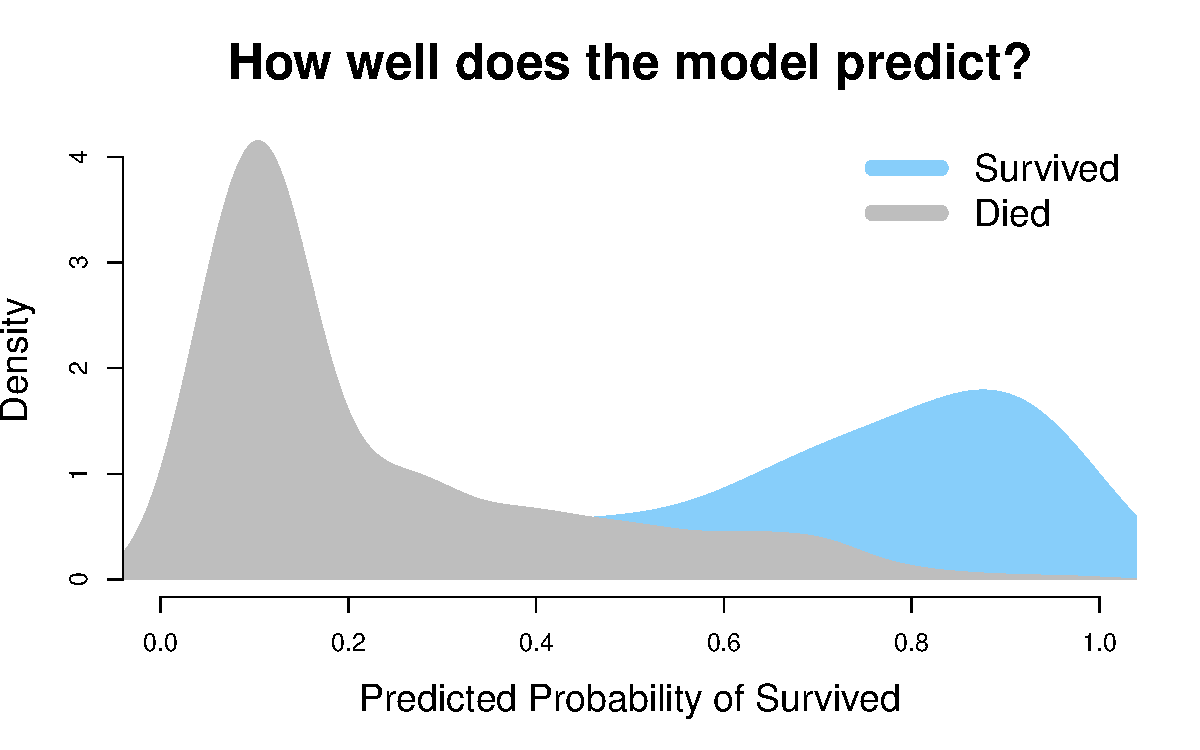
\includegraphics[scale=0.35]{titanic_prediction_dens.pdf}

\end{column}
\end{columns}

\end{frame}

%@@@@@@@@@@@@@@@@@@@@@@@@@@@@@@@@@@@@@@@@@@@@@@@@@
\begin{frame}
\frametitle{Logistic Regression: confusion matrix}

\begin{columns}
\begin{column}{0.5\textwidth}

\begin{itemize}
\item We could measure model fit by aggregating TP/TN/FP/FN across the entire data set;
\bigskip
\bigskip

\item Add each of these up across the data:
\begin{align*}
\begin{array}{cccc}
&&\mbox{Prediction}&\\
&&\mbox{Survived}&\mbox{Died}\\
\mbox{Observation}&\mbox{Survived}&239&103\\
&\mbox{Died}&73&472\\
\end{array}
\end{align*}

\end{itemize}

\end{column}
\begin{column}{0.5\textwidth}

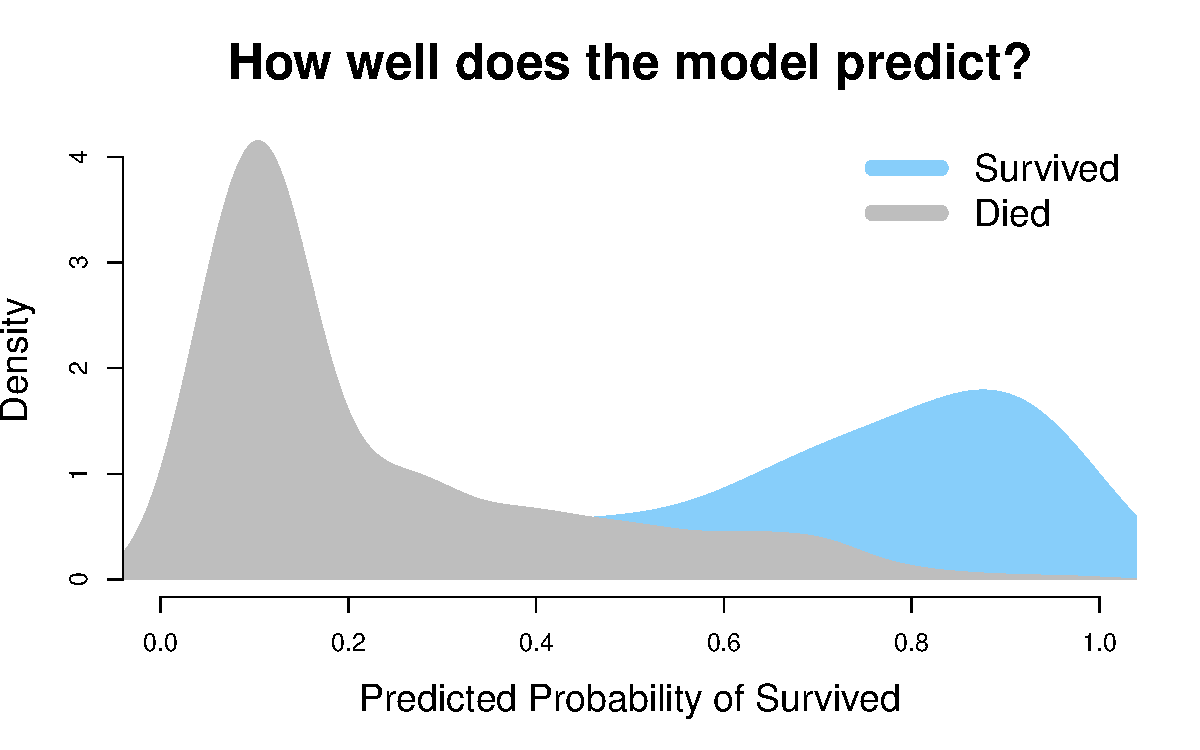
\includegraphics[scale=0.35]{titanic_prediction_dens.pdf}

\end{column}
\end{columns}

\end{frame}

%@@@@@@@@@@@@@@@@@@@@@@@@@@@@@@@@@@@@@@@@@@@@@@@@@
\begin{frame}
\frametitle{Logistic Regression: accuracy}

\begin{columns}
\begin{column}{0.5\textwidth}

\begin{itemize}
\item We could measure model fit by summarizing the confusion matrix up as a single number;
\bigskip
\bigskip

\item One way to do this is by using \textbf{accuracy}:
\begin{align*}
\frac{TP + TN}{TP + TN + FP + FN}
\end{align*}
\bigskip

\item[]\color{white} Beware!  Accuracy is only useful when each value of the dependent variable is equally important.

\end{itemize}

\end{column}
\begin{column}{0.5\textwidth}

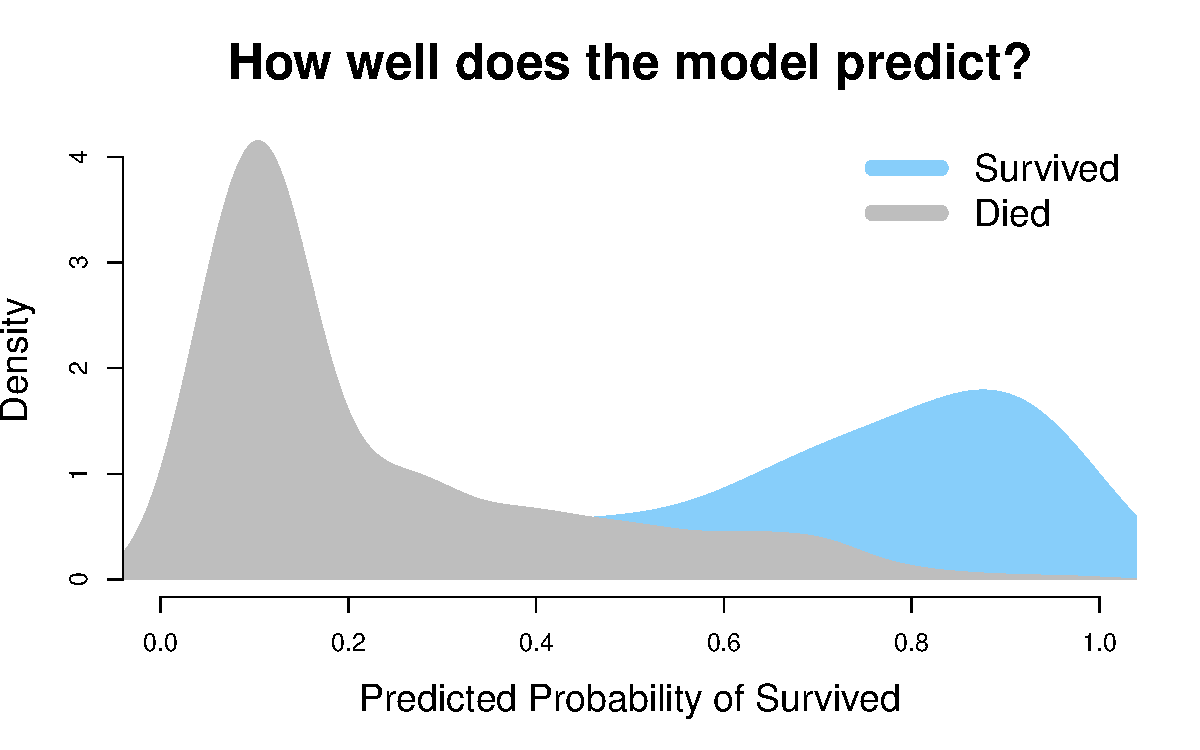
\includegraphics[scale=0.35]{titanic_prediction_dens.pdf}

\end{column}
\end{columns}

\end{frame}

%@@@@@@@@@@@@@@@@@@@@@@@@@@@@@@@@@@@@@@@@@@@@@@@@@
\begin{frame}
\frametitle{Logistic Regression: accuracy}

\begin{columns}
\begin{column}{0.5\textwidth}

\begin{itemize}
\item We could measure model fit by summarizing the confusion matrix up as a single number;
\bigskip
\bigskip

\item One way to do this is by using \textbf{accuracy}:
\begin{align*}
\frac{239 + 472}{239 + 472 + 73 + 103}\approx 0.8016;
\end{align*}
\bigskip

\item[]\color{white} Beware!  Accuracy is only useful when each value of the dependent variable is equally important.

\end{itemize}

\end{column}
\begin{column}{0.5\textwidth}

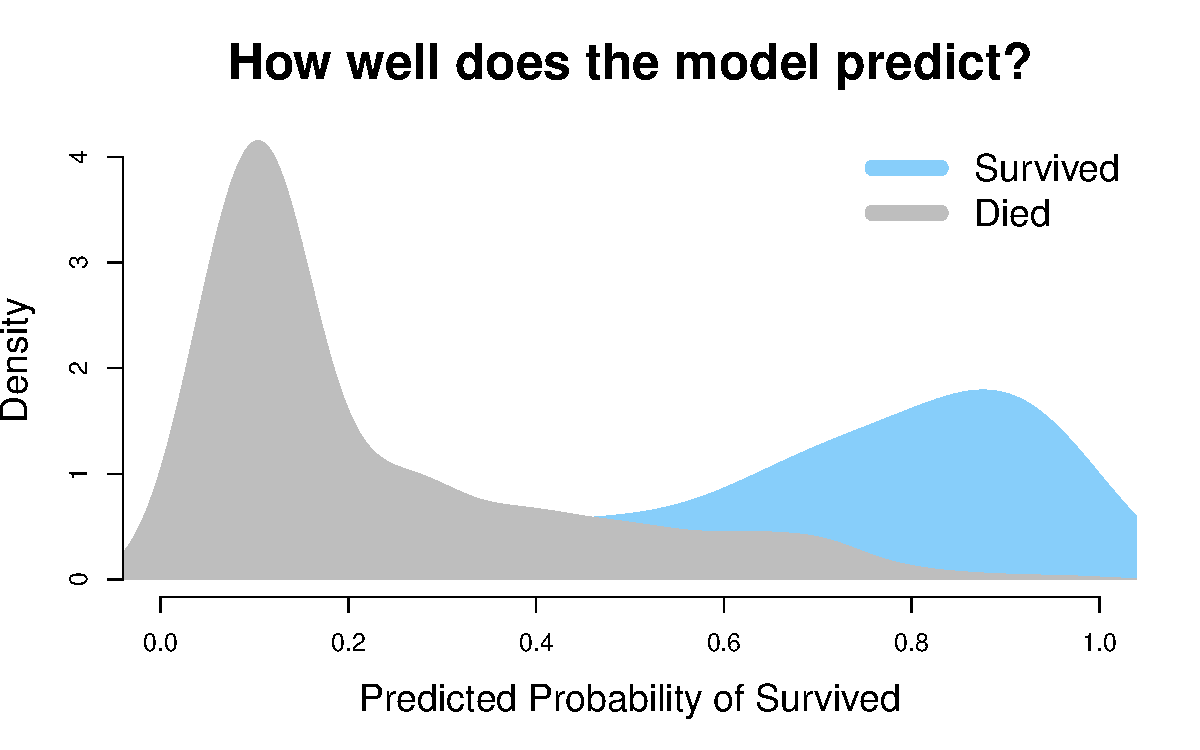
\includegraphics[scale=0.35]{titanic_prediction_dens.pdf}

\end{column}
\end{columns}

\end{frame}

%@@@@@@@@@@@@@@@@@@@@@@@@@@@@@@@@@@@@@@@@@@@@@@@@@
\begin{frame}
\frametitle{Logistic Regression: accuracy}

\begin{columns}
\begin{column}{0.5\textwidth}

\begin{itemize}
\item We could measure model fit by summarizing the confusion matrix up as a single number;
\bigskip
\bigskip

\item One way to do this is by using \textbf{accuracy}:
\begin{align*}
\frac{239 + 472}{239 + 472 + 73 + 103}\approx 0.8016;
\end{align*}
\bigskip

\item Beware!  Accuracy is only useful when each value of the dependent variable is equally important.

\end{itemize}

\end{column}
\begin{column}{0.5\textwidth}

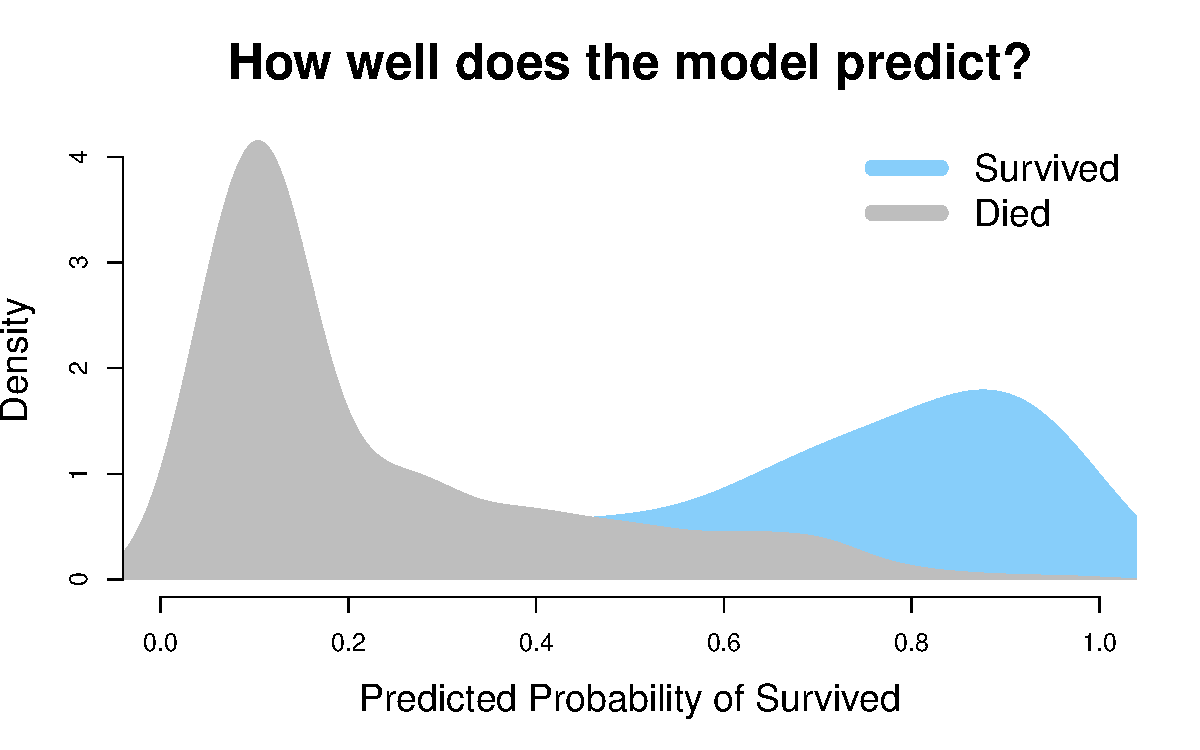
\includegraphics[scale=0.35]{titanic_prediction_dens.pdf}

\end{column}
\end{columns}

\end{frame}

%@@@@@@@@@@@@@@@@@@@@@@@@@@@@@@@@@@@@@@@@@@@@@@@@@
\begin{frame}
\frametitle{Logistic Regression: recall/precision}

\begin{columns}
\begin{column}{0.5\textwidth}

\begin{itemize}
\item We could measure model fit by trying to gauge its ability to identify the survivors and only the survivors;
\bigskip

\item \textbf{Recall}: of all the survivors how many did the model identify?
\begin{align*}
R = \frac{TP}{TP + FN}
\end{align*}

\item \textbf{Precision}: of all the passengers predicted to survive how many actually did?
\begin{align*}
P = \frac{TP}{TP + FP}.
\end{align*}
\bigskip

\end{itemize}

\end{column}
\begin{column}{0.5\textwidth}

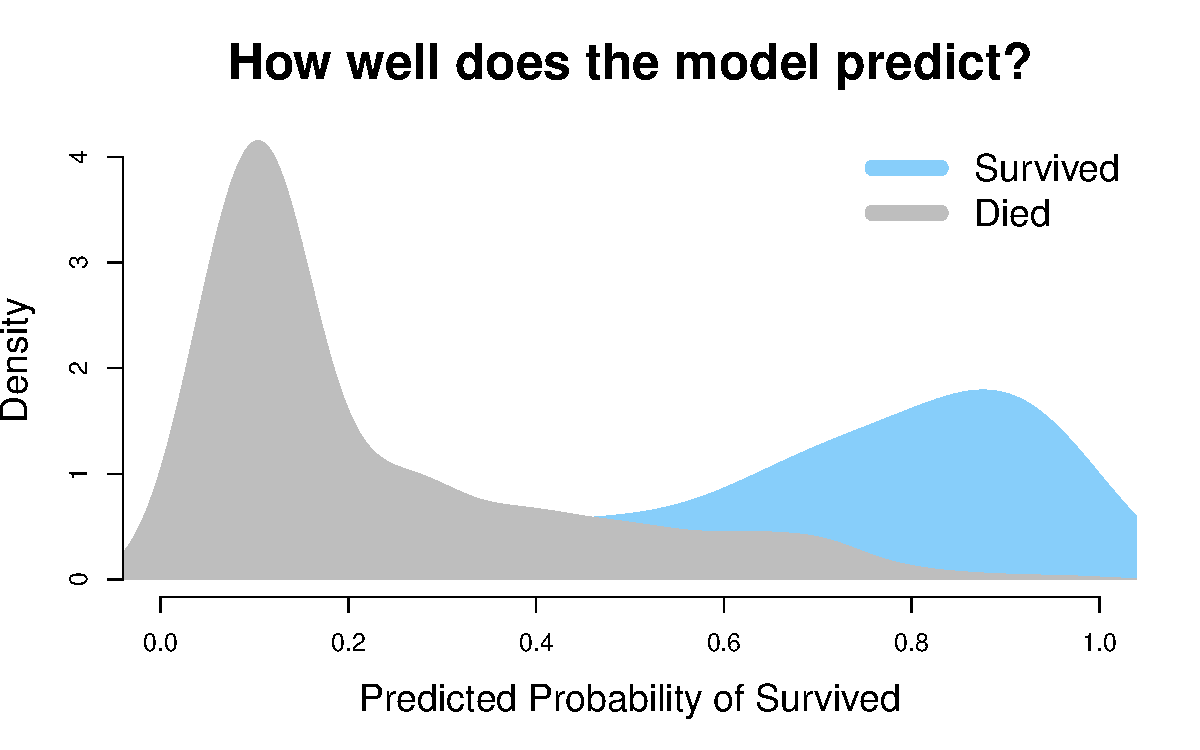
\includegraphics[scale=0.35]{titanic_prediction_dens.pdf}

\end{column}
\end{columns}

\end{frame}

%@@@@@@@@@@@@@@@@@@@@@@@@@@@@@@@@@@@@@@@@@@@@@@@@@
\begin{frame}
\frametitle{Logistic Regression: recall/precision}

\begin{columns}
\begin{column}{0.5\textwidth}

\begin{itemize}
\item We could measure model fit by trying to gauge its ability to identify the survivors and only the survivors;
\bigskip

\item \textbf{Recall}: of all the survivors how many did the model identify?
\begin{align*}
R = \frac{239}{239 + 103}\approx 0.70
\end{align*}

\item \textbf{Precision}: of all the passengers predicted to survive how many actually did?
\begin{align*}
P = \frac{239}{239 + 73} \approx 0.77.
\end{align*}
\bigskip

\end{itemize}

\end{column}
\begin{column}{0.5\textwidth}

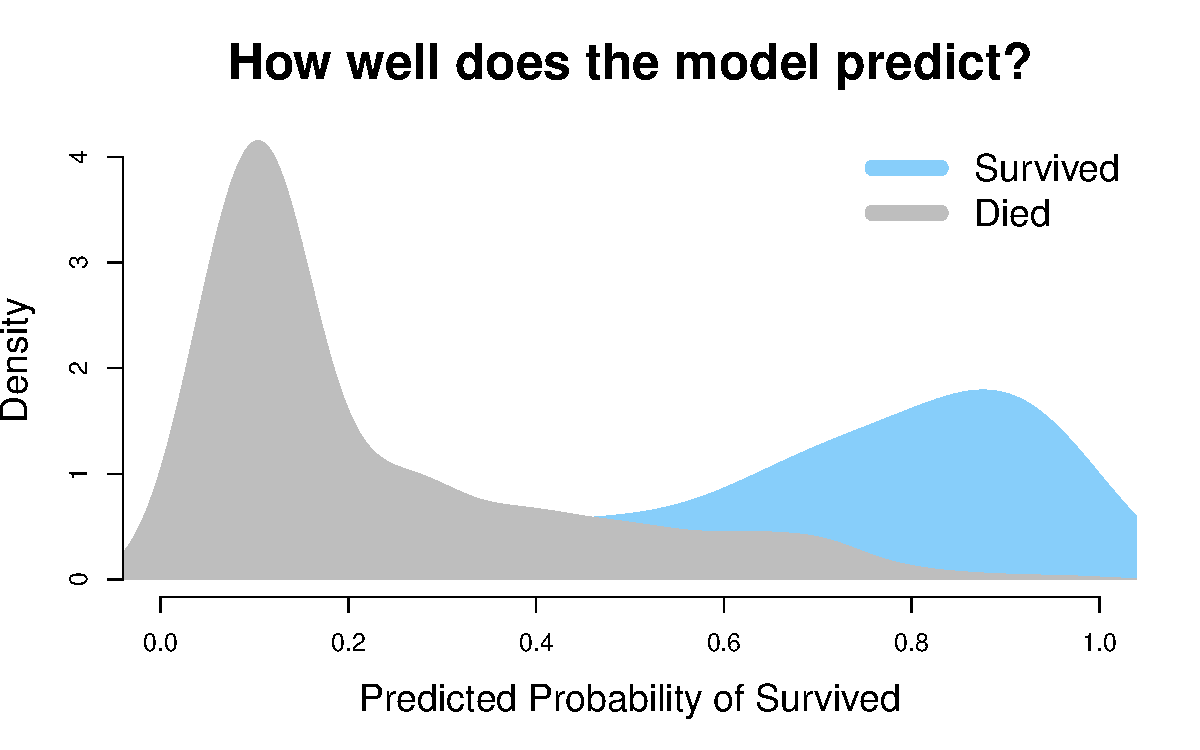
\includegraphics[scale=0.35]{titanic_prediction_dens.pdf}

\end{column}
\end{columns}

\end{frame}

%@@@@@@@@@@@@@@@@@@@@@@@@@@@@@@@@@@@@@@@@@@@@@@@@@
\begin{frame}

\begin{center}
\Huge\textbf{Why should we care?}\\
\bigskip
\bigskip
\large Better model fit $=$ better prediction $=$ a more useful, impactful model.\\
\end{center}

\end{frame}



\end{document}






